% Figure: Segment structure diagram
\begin{center}
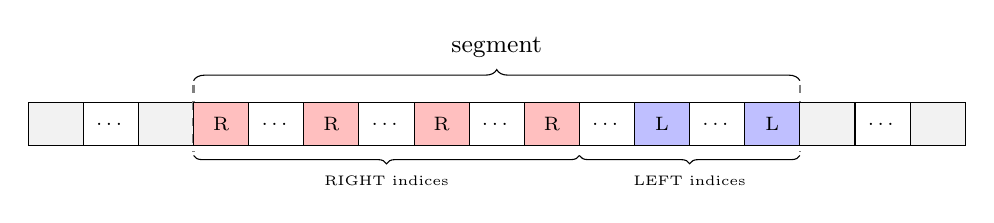
\begin{tikzpicture}[
    cell/.style={minimum width=0.7cm, minimum height=0.55cm, draw, font=\scriptsize},
    dotcell/.style={cell, fill=white},
    right/.style={cell, fill=red!25},
    left/.style={cell, fill=blue!25},
    clean/.style={cell, fill=gray!10},
    boundary/.style={dashed, thick, black!50}
]
% Clean elements before (attached to segment)
\node[clean] (c0) at (0, 0) {};
\node[dotcell] at (0.7, 0) {\dots};
\node[clean] (c1) at (1.4, 0) {};

% Segment boundary (between c1 and r1)
\draw[boundary] (1.75, 0.5) -- (1.75, -0.35);

% R/M region: R ... M ... R ... M
\node[right] (r1) at (2.1, 0) {R};
\node[dotcell] at (2.8, 0) {\dots};
\node[right] (r2) at (3.5, 0) {R};
\node[dotcell] at (4.2, 0) {\dots};
\node[right] (r3) at (4.9, 0) {R};
\node[dotcell] at (5.6, 0) {\dots};
\node[right] (r4) at (6.3, 0) {R};

% L region: ... L ... L
\node[dotcell] at (7.0, 0) {\dots};
\node[left] (l1) at (7.7, 0) {L};
\node[dotcell] at (8.4, 0) {\dots};
\node[left] (l2) at (9.1, 0) {L};

% Segment boundary (between l2 and c2)
\draw[boundary] (9.45, 0.5) -- (9.45, -0.35);

% Clean elements after (attached to segment)
\node[clean] (c2) at (9.8, 0) {};
\node[dotcell] at (10.5, 0) {\dots};
\node[clean] (c3) at (11.2, 0) {};

% Braces
\draw[decorate, decoration={brace, amplitude=4pt}] 
    (1.75, 0.55) -- (9.45, 0.55) node[midway, above=5pt, font=\small] {segment};
\draw[decorate, decoration={brace, amplitude=3pt, mirror}] 
    (1.75, -0.4) -- (6.65, -0.4) node[midway, below=4pt, font=\tiny] {RIGHT indices};
\draw[decorate, decoration={brace, amplitude=3pt, mirror}] 
    (6.65, -0.4) -- (9.45, -0.4) node[midway, below=4pt, font=\tiny] {LEFT indices};
\end{tikzpicture}
\end{center}
